% !TEX root = ../../lectures.tex
\section{From Linear to Non-Linear: The Formation of Shock Waves}

This section aims to qualitatively illustrate how the formation of shock waves is a natural and, consequently, a frequent phenomenon in astrophysical environments.

In the linear regime, small perturbations in a medium propagate at the sound speed, \( c_{s,0} \), which we earlier defined in terms of the pressure \( P_0 \) and density \( \rho_0 \) of the medium (see equation~\ref{eq:cs02}). For linear waves, \( c_{s,0} \) is assumed to be constant across the medium. 

When the amplitude of the perturbation increases, the wave enters the non-linear regime, where the propagation speed depends on the local density. Specifically:  
\[
c_s^2 \propto \frac{P}{\rho} \propto \rho^{\gamma - 1},
\]  
where \( \gamma \sim 5/3 \) is the adiabatic index of the medium. \emph{High-density regions propagate faster than low-density regions}. 
%
This effect fundamentally alters the wave's behavior.  

Imagine a sinusoidal wave (as the solution found in equation~\ref{eq:rhowaveform}) traveling through a medium. As density peaks (crests) move faster than the troughs, the waveform becomes increasingly asymmetric. Over time, this leads to the steepening of the wave front until the crest overtakes the trailing edge. At this point, the wave profile develops a physical inconsistency --- a \emph{multi-valued} solution (see figure~\ref{fig:landau}). The resolution to this breakdown is the formation of a \emph{shock wave}, a discontinuity in the fluid properties.

As a direct consequence of their formation process, shock waves exhibit several distinctive properties:
%
\begin{itemize}
\item Shock waves are associated with matter moving at speeds exceeding the local sound speed. This supersonic motion compresses and heats the medium, creating a steep discontinuity.  
\item The medium cannot adjust to changes induced by the shock wave fast enough. As a result, fluid variables such as density, temperature, and velocity undergo abrupt \emph{jumps} at the shock front.  
\item The shock propagates faster than any signal can travel within the medium. Consequently, regions ahead of the shock (pre-shock) remain unaware of the disturbance until the shock front reaches them.  
\end{itemize}

\begin{figure}[!t]
\centering
\includegraphics[width=0.45\textwidth]{figures/shocklandau.pdf}
\caption{}
\label{fig:landau}
\end{figure}

In fact, shock waves are a ubiquitous feature in astrophysical environments, reflecting the variety of processes that drive supersonic motion. 
%
Notable examples include:
\begin{itemize}
\item Fast stellar winds collide with the interstellar medium, forming bow shocks or termination shocks.  
\item Supernova blast waves plow into the surrounding medium.  
\item In gamma-ray bursts, colliding relativistic shells generate shocks within the ejecta.  
\item Matter falling onto compact objects like neutron stars or black holes forms accretion shocks.  
\item Shock waves develop as material accretes onto galaxy clusters' hydrostatic intracluster medium.  
\end{itemize}

Their presence in is a testament to the dynamic, high-energy processes shaping the universe.

\section{Interstellar Shock Waves}

\begin{figure}[!t]
\centering
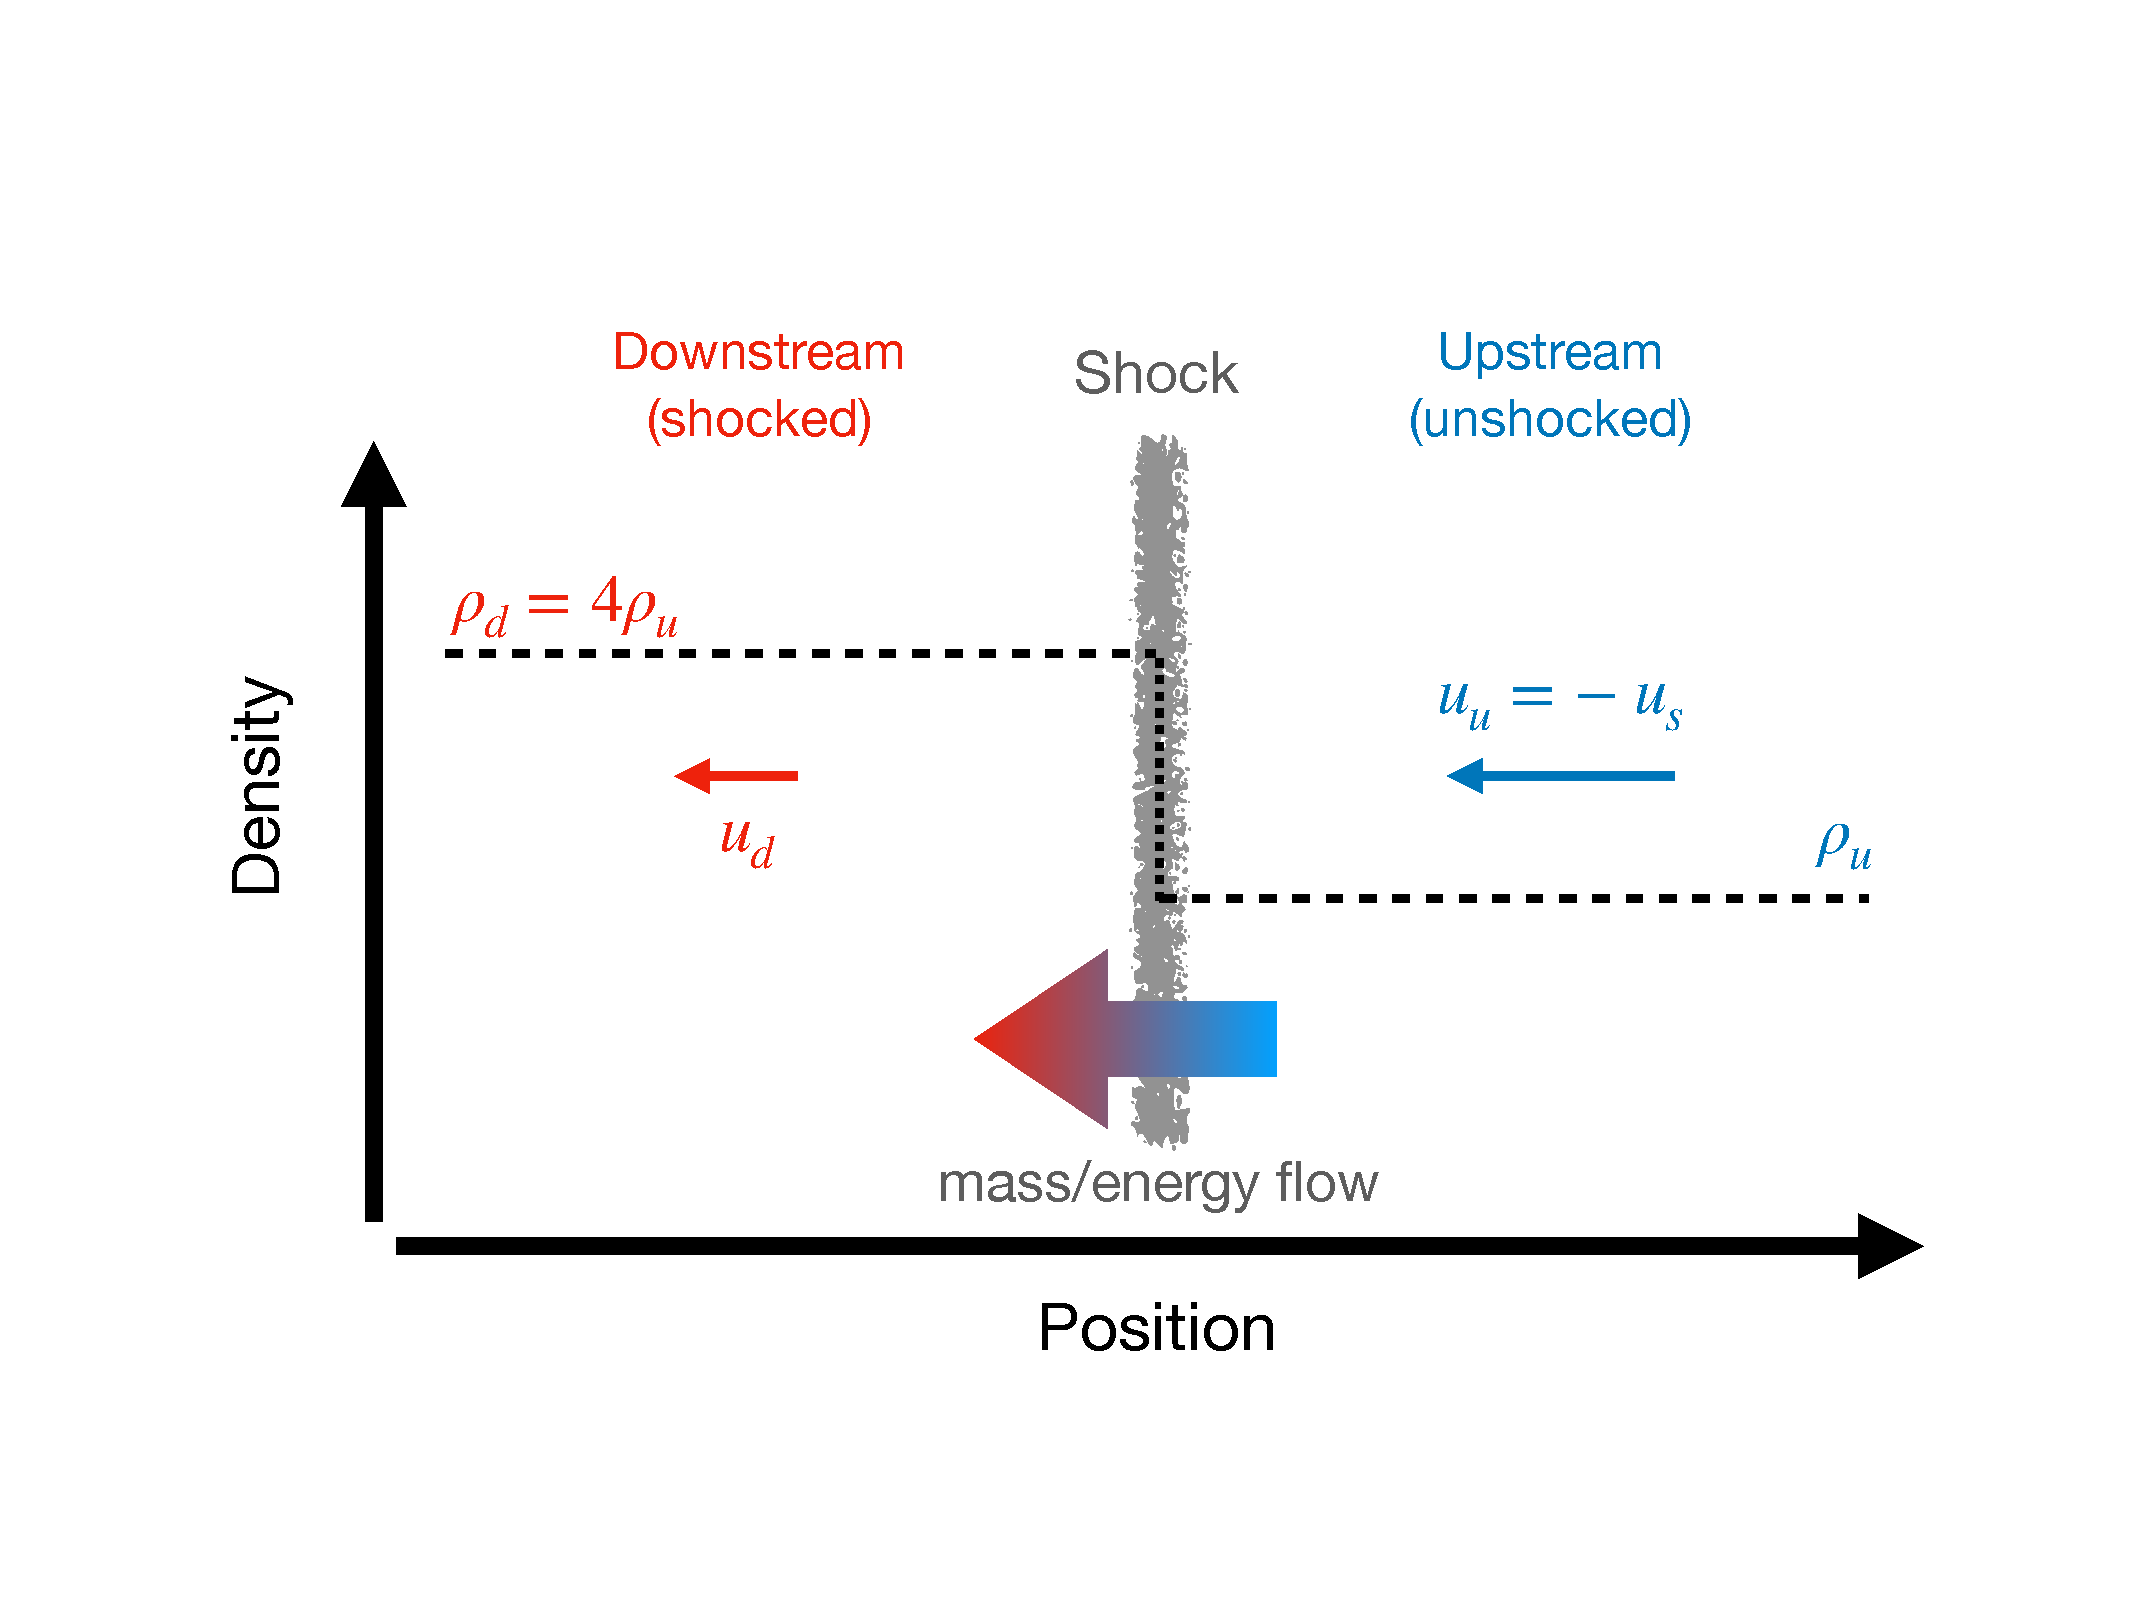
\includegraphics[width=0.57\textwidth]{figures/shockflow.pdf}
\caption{}\label{fig:shockflow}
\end{figure}

In hydrodynamics, solutions often feature \emph{discontinuous} behavior, meaning physical quantities - such as density, pressure, or velocity - can change abruptly across certain surfaces. Mathematically, this manifests as distinct values when approaching the discontinuity from either side. However, in the physical world, these changes are not infinitely sharp as suggested by idealized mathematical models. Instead, the transition occurs over a region that is small relative to all other relevant physical scales.

A \emph{shock} is a particular type of discontinuity characterized by a surface that separates two fluid regions with contrasting properties. Crucially, this surface allows the transfer of mass, momentum, and energy across it (see Figure~\ref{fig:shockflow}). Shocks naturally arise in the non-linear regime of hydrodynamics, including magnetohydrodynamics, as seen in the previous section. 

In astrophysics, shocks are of immense importance because they dramatically alter the physical state of the gas. For instance, post-shock gas often emits significantly more radiation than pre-shock gas, making shocks detectable phenomena.

Astrophysical shocks differ fundamentally from their terrestrial counterparts due to the nature of particle interactions. Under standard atmospheric conditions - where the particle number density is approximately \( n \sim 10^{23} \, \text{cm}^{-3} \) and the collision cross-section is \( \sigma \sim \pi r_A^2 \sim 10^{-16} \, \text{cm}^2 \) (with \( r_A \sim 65 \, \text{pm} \), the atomic radius of nitrogen) - the mean free path of a particle is very short, about \( \lambda \simeq 1 / (n \sigma) \sim 10^{-7} \, \text{cm} \). Frequent collisions in this regime efficiently convert ordered kinetic energy into disordered thermal energy, leading to the formation of a \emph{collisional shock}.

Astrophysical environments, however, present a vastly different picture. Most particles in these regions are ionized, and the cross-sections for interactions between charged particles are orders of magnitude smaller, typically \( \sigma \sim \pi r_0^2 \sim 3 \times 10^{-25} \, \text{cm}^2 \), where \( r_0 \sim 6 \, \text{fm} \) represents the nuclear radius. Additionally, the particle number density in these environments is exceedingly low, around \( n \sim 1 \, \text{cm}^{-3} \). This results in an enormous mean free path, on the order of megaparsecs.

Given these conditions, shocks in astrophysical settings are predominantly \emph{collisionless}. Their formation and energy dissipation mechanisms do not rely on direct particle collisions or Coulomb interactions. Instead, these processes are governed by collective interactions mediated by the ambient magnetic and electric fields, which play a central role in shock dynamics and energy dissipation.

The detailed microphysics of astrophysical shocks are intricate and extend beyond the scope of these lectures. Factors like finite conductivity and plasma instabilities determine the size and structure of the shock transition region. However, despite these complexities at the microscopic level, the conservation laws of mass, momentum, and energy continue to hold and provide a robust framework for understanding shocks at macroscopic scales.

For non-relativistic shock waves, it is helpful to first define a reference frame. In the \emph{Galaxy frame}, the unshocked medium (ISM) is at rest, and the shock propagates through it at a speed \( u^\prime_s \). In this frame, the shocked gas moves at a slower speed, \( u^\prime_d (< u^\prime_s) \), behind the shock front.

However, a more convenient perspective is the \emph{shock front frame}, where the discontinuity surface itself is stationary (\( u_s = 0 \)). In this frame, the upstream medium approaches the shock at a velocity \( u_u = -u^\prime_s \), while the downstream shocked gas recedes from the shock at \( u_d = u^\prime_s - u^\prime_d \). The relative speed between the upstream and downstream fluids is thus \( u_{\text{rel}} = u_d - u_u \). \TODO{check}

Throughout our discussion, we will adopt the shock front frame to simplify calculations and interpretations. In this frame, we categorize physical quantities based on their location relative to the shock. Quantities \emph{upstream} of the shock (before the discontinuity) are labeled with the subscript 'u,' while those \emph{downstream} of the shock (after the discontinuity) are labeled with the subscript 'd.'

In the study of shock dynamics, we focus on key thermodynamic quantities - density, pressure, temperature, and momentum - on either side of the shock (upstream and downstream). To analyze these quantities, we employ conservation equations in the general form \( \frac{dJ}{dz} = 0 \), where \( J \) represents the flux of a conserved quantity, such as mass, energy, or momentum.

This conservation principle implies that the net flux across the shock remains constant. Integrating this over a small region surrounding the shock yields:
%
\[
\int_{-\epsilon}^{\epsilon} \frac{dJ}{dx} \, dx = J_d - J_u = 0,
\]
%
where \( J_d \) and \( J_u \) denote the downstream and upstream fluxes, respectively. To simplify notation, we write this as \( [J]_{\text{sh}} = J_d - J_u = 0 \), emphasizing that there is no net change in the flux across the shock.

Next, we summarize the key conservation equations for a fluid, assuming that the only force acting is the pressure gradient \( \nabla P \), and neglecting effects from magnetic fields or gravity:
%
\begin{itemize}  
\item The equation of mass conservation is given by:
   \begin{equation}
   \frac{\partial \rho}{\partial t} + \nabla \cdot (\rho \vec{u}) = 0~,
   \end{equation}
   where \( \rho \) is the fluid density and \( \vec{u} \) is the velocity field. This ensures that mass is neither created nor destroyed within the system.

\item Conservation of momentum per unit volume is expressed as:
   \begin{equation}
   \rho \frac{\partial \vec{u}}{\partial t} + \rho (\vec{u} \cdot \nabla) \vec{u} = -\nabla P,
   \end{equation}
   which accounts for the balance between inertial forces and pressure gradients in the fluid.

\item The conservation of energy per unit volume can be written as:
   \begin{equation}
   \frac{\partial}{\partial t} \left( \frac{1}{2} \rho u^2 + \rho U \right) + \nabla \cdot \left[ \vec{u} \left( \frac{1}{2} \rho u^2 + \rho U + P \right) \right] = 0,
   \end{equation}
   where \( U \) is the specific internal energy, and \( \epsilon = \rho U \) represents the internal energy per unit volume.
\end{itemize}

\TODO{Why P?}

To simplify the analysis, we focus on a one-dimensional (planar) shock in a steady state (\( \partial_t = 0 \)) within the reference frame where the shock is stationary. 
%
Under these conditions:
\begin{itemize}
\item The mass continuity equation reduces to:
   \begin{equation}
   \frac{\partial}{\partial z} (\rho u) = 0,
   \end{equation}
   indicating that the mass flux \( \rho u \) is constant across the shock.

\item Substituting the mass continuity equation into the momentum equation yields:
\begin{equation}
\rho u \frac{\partial u}{\partial z} = -\frac{\partial P}{\partial z} \quad \rightarrow \quad \frac{\partial}{\partial z} (P + \rho u^2) = 0.
\end{equation}
Here, the total pressure \( P + \rho u^2 \) (comprising gas pressure and the dynamic pressure) is conserved across the shock.

\item Similarly, the energy conservation law in the steady state provides constraints on the total energy flux, incorporating both kinetic and internal energy terms:
%
\begin{equation}
\frac{\partial}{\partial z} \left( \rho u \left[ \frac{1}{2} u^2 + U + \frac{P}{\rho} \right] \right) = 0 
\end{equation}
%
Simplifying further, and expressing the equation in terms of the adiabatic index \( \gamma \) (see Appendix~\ref{app:thermo}), we arrive at:
%
\begin{equation}
\frac{\partial}{\partial z} \left( \frac{1}{2} u^2 + \frac{\gamma}{\gamma - 1}\frac{P}{\rho} \right) = 0 
\end{equation}
\end{itemize}

% in terms of specific enthalpy \( w \) (see Appendix):
%
%\begin{equation}
%w = U + \frac{P}{\rho} = \frac{\gamma}{\gamma - 1}\frac{P}{\rho}
%\end{equation}

To summarize, under the assumption of planar geometry and in the shock frame, the conservation of mass, momentum, and energy fluxes across the shock can be expressed as follows:

\begin{remark}
\begin{eqnarray}
\left[ \rho u \right]_{\rm sh} & = & 0, \label{eq:RH1} \\
\left[ \rho u^2 + P \right]_{\rm sh} & = & 0, \label{eq:RH2} \\
\left[ \frac{1}{2} u^2 + \frac{\gamma}{\gamma - 1} \frac{P}{\rho} \right]_{\rm sh} & = & 0, \label{eq:RH3}
\end{eqnarray}
\end{remark}

These equations are collectively known as the \emph{Rankine-Hugoniot jump conditions}~\cite{}. They serve as the fundamental dynamical equations governing shocks, encapsulating the conservation laws across the discontinuity. Essentially, they establish the relationships between physical quantities - density, pressure, and velocity - on either side of the shock front.

In this framework, we are tasked with solving for three unknowns, corresponding to the post-shock quantities, while having three equations at our disposal. Besides the trivial solution, where all quantities remain unchanged across the shock, our goal is to derive the non-trivial solution that describes the physical changes induced by the shock. This solution characterizes the downstream state in terms of upstream conditions and the properties of the shock.

To proceed, we recall the definition of the sound speed, which is given by:
%
\begin{equation}
c_{\text{s}} = \left( \frac{\partial P}{\partial \rho} \right)^{1/2} = \left(\frac{\gamma P}{\rho}\right)^{1/2}.
\end{equation}

Here, we assume the gas behaves as an ideal gas, with the equation of state \( P = K \rho^\gamma \), where \( \gamma \) is the adiabatic index, or the ratio of specific heats. For a monoatomic gas, in particular, \( \gamma = 5/3 \).

We then introduce the \emph{Mach number}, which quantifies the ratio of the shock speed to the local sound speed in a given region \( i \). This is defined as:
%
\begin{equation}
\mathcal{M}_i = \frac{v_i}{c_{\text{s},i}},
\end{equation}
%
where \( v_i \) is the velocity of the fluid relative to the shock front, and \( c_{\text{s},i} \) is the local sound speed. Using this definition, the momentum flux equation can be expressed as:
%
\begin{equation}
\rho_i u_i^2 + P_i = \rho_i c_{\text{s}, i}^2 \left( \frac{u_i^2}{c_{\text{s},i}^2} \right) + P_i = (1 + \gamma \mathcal{M}_i^2) P_i.
\end{equation}

If we fix the upstream properties \( \rho_u \), \( u_u \), and \( P_u \), the conservation equations (\ref{eq:RH1})-(\ref{eq:RH3}) can be solved to determine the corresponding downstream quantities \( \rho_d \), \( u_d \), and \( P_d \). The solutions are summarized as (see Appendix~\ref{app:RH} for details):
%
\begin{itemize}
\item Density Compression Ratio:  
\begin{equation}
\frac{\rho_d}{\rho_u} = \frac{u_u}{u_d} = \frac{(\gamma + 1) \mathcal{M}_u^2}{(\gamma - 1) \mathcal{M}_u^2 + 2}~.
\end{equation}

\item Pressure Ratio:
\begin{equation}
\frac{P_d}{P_u} = \frac{2\gamma \mathcal{M}_u^2}{\gamma + 1} - \frac{\gamma - 1}{\gamma + 1}~.
\end{equation}

\item Temperature Ratio:
\begin{equation}
\frac{T_d}{T_u} = \frac{\left[ 2\gamma \mathcal{M}_u^2 - (\gamma - 1) \right] \left[ (\gamma - 1) \mathcal{M}_u^2 + 2 \right]}{(\gamma + 1)^2 \mathcal{M}_u^2}~.
\end{equation}
\end{itemize}

Under the assumption of \emph{strong shock conditions}, where \( \mathcal{M}_u \gg 1 \), and considering a monoatomic gas with \( \gamma = 5/3 \), we can derive a simplified expression for the jump in density across the shock:
%
\begin{remark}
\begin{equation}
r = \frac{\rho_d}{\rho_u} = \frac{u_u}{u_d} \, \underset{\mathcal{M} \gg 1}{\longrightarrow} \, \frac{\gamma + 1}{\gamma - 1} \simeq 4,
\end{equation}
\end{remark}
%
where \( r \) represents the \emph{compression factor}.

This result highlights the maximum compression achievable under the conditions of a strong shock, which depends solely on the adiabatic index \( \gamma \). For \( \gamma = 5/3 \), characteristic of a monoatomic gas, the compression factor reaches its theoretical limit of 4. It is important to note that this upper bound arises due to the constraints imposed by the conservation equations and the nature of the ideal gas equation of state.

Similarly, for the pressure jump across the shock, we have:
%
\begin{equation}
\frac{P_d}{P_u} \, \underset{\mathcal{M} \gg 1}{\longrightarrow} \, \frac{2 \gamma}{\gamma + 1} \mathcal{M}_u^2 \simeq \frac{5}{4} \mathcal{M}_u^2.
\end{equation}

This relation shows that the post-shock pressure grows quadratically with the upstream Mach number, indicating that strong shocks are highly efficient at compressing and heating the gas.

In the shock frame, the upstream gas approaches the shock front with velocity \( u_u \), while the downstream velocity \( u_d \) is significantly reduced. For a strong shock with \( \gamma = 5/3 \), the relationship \( u_d \approx \frac{1}{4}u_u \) holds. This deceleration results in an increase in density and pressure as the kinetic energy of the plasma is converted into thermal energy.

However, energy conservation dictates that the kinetic energy lost during the shock transition must transform into \emph{heat}, resulting in a significant increase in the downstream temperature. Examining the temperature ratio \( T_d / T_u \) under strong shock conditions, we find:
%
\begin{equation}
\frac{T_d}{T_u}  \, \underset{\mathcal{M} \gg 1}{\longrightarrow} \, \frac{2 \gamma (\gamma - 1)}{(\gamma +1)^2} \mathcal{M}_u^2.
\end{equation}

By substituting the upstream Mach number \( \mathcal{M}_u^2 = u_u^2 / c_{\text{s},u}^2 \), the downstream temperature can be expressed as:
%
\begin{equation}
k_B T_d = k_B T_u \frac{2 \gamma (\gamma - 1)}{(\gamma + 1)^2} \frac{u_u^2}{c_{\text{s},u}^2}.
\end{equation}

Using the thermodynamic relationships \( c_{\text{s},i}^2 = \gamma P_i / \rho_i \), \( \rho_i = n_i m_p \), and \( P_i = n_i k_B T_i \), into this expression yields:
%
\begin{remark}
\begin{equation}
{\color{red}k_B T_d} = {\color{blue}\frac{3}{16} m_p u_u^2}~.
\end{equation}
\end{remark}

This result demonstrates that \emph{shocks efficiently convert the {\color{blue}bulk kinetic energy of the upstream medium} into {\color{red}thermal (internal) energy in the downstream region}}. 

For typical astrophysical shocks, where upstream velocities \( u_u \gtrsim 10^4 \, \text{km/s} \), the downstream temperature can reach values on the order of \( T_d \sim 10^7 \, \text{K} \). 
%
This heating mechanism explains the radiative signatures - often in the X-ray or higher-energy bands - of shocked plasmas in various astrophysical phenomena.

In summary, as the plasma crosses the shock front, it is:
\begin{remark}
\begin{description}
\item[Compressed:] \( \rho_d = 4 \rho_u \)
\item[Decelerated:] \( v_d = \frac{1}{4} v_u \)
\item[Heated:] \( T_d \ll T_u \)
\end{description}
\end{remark}

The transformation of inflowing kinetic energy into thermal energy in shock waves is inherently tied to the generation of \emph{entropy}. This transformation arises from the dissipation of ordered bulk kinetic energy - where particle velocities are aligned - into disordered internal kinetic energy, or heat. In classical settings, this dissipation is facilitated by particle collisions within the shock wave.
%
However, as previously discussed, the mean free path for collisions in astrophysical environments can be macroscopically large, often exceeding the size of the system. Under such conditions, direct particle collisions become ineffective as a mechanism for energy dissipation. Instead, energy exchange is mediated by \emph{electromagnetic fields}.

In collisionless shocks, the effective thickness of the shock is governed by the scale over which particles interact with the magnetic fields. This scale is typically associated with the \emph{non-relativistic Larmor radius} of a proton.

For a proton with a velocity of \( v \sim 10^4 \, \text{km/s} \) (typical of a supernova explosion) moving within a galactic magnetic field of \( B \sim 1 \, \mu\text{G} \), the Larmor radius \( r_{\text{B}} \) is given by:
%
\[
r_{\text{B}} = \frac{m_p v c}{e B} \simeq 10^{10} \, \text{cm}~.
\]

To put this into perspective, the typical length scales of supernova (SN) explosions are on the order of a parsec. The thickness of the shock layer, characterized by the Larmor radius, is therefore many orders of magnitude smaller than the overall scale of the system. 
%
This vast difference in scales justifies the common approximation in astrophysical modeling that the shock is an \emph{infinitely thin layer}. 

\TODO{entropy}

%The transformation of inflow kinetic energy into thermal energy in shock waves is accompanied by the generation of entropy. The key to this transformation is the collisions among particles within the shock wave. These collisions convert the ordered bulk kinetic energy, where particle velocities are aligned, into disordered internal kinetic energy, or heat.
%
%However, as we have previously noted, the mean free path for collisions in astrophysical conditions can be macroscopically large. In such scenarios, energy exchange among particles is mediated by electromagnetic fields.
%%
%Therefore, the thickness of the shock is more characterized by the non-relativistic Larmor radius of a proton. This radius reflects the scale over which particles are deflected by the magnetic field present at the shock front.
%
%Considering a typical proton velocity of \( \sim 10^4 \) km/s in a supernova explosion, and within a typical galactic magnetic field of \( 1 \mu \)G, the Larmor radius (\( r_{\text{B}} \)) is calculated as:
%%
%\begin{equation}
%r_{\text{B}} = \frac{m_p v c}{e B} \simeq 10^{10}~\text{cm}
%\end{equation}
%
%When compared to typical lengths involved in supernova (SN) explosions, which are on the order of a parsec (see later), the shock thickness is several orders of magnitude smaller. Therefore, in the grand scale of such astrophysical phenomena, the approximation of an infinitely thin shock layer is justified.
%
%Finally, we want to compute the post-shock Mach number \( M_2 \):
%%
%\begin{equation}
%\mathcal M_2 = \frac{u_2}{c_{\rm s,2}} = \mathcal M_1 \frac{u_2}{u_1} \frac{c_1}{c_2} = \mathcal M_1 \frac{u_2}{u_1} \left( \frac{T_1}{T_2} \right)^{1/2}
%\end{equation}
%%
%in the strong shock limit:
%%
%\begin{equation}
%\mathcal M_2 = \mathcal M_1 \frac{\gamma - 1}{\gamma + 1} \left[ \frac{(\gamma + 1)^2}{2\gamma(\gamma - 1) \mathcal M_1^2} \right]^{1/2} = \left( \frac{\gamma - 1}{2\gamma} \right)^{1/2} \simeq 0.45 
%\end{equation}
%%
%so a shock converts supersonic gas into subsonic gas.
%%
%In doing so, it increases the specific entropy of the gas by an amount~(see appendix):
%%
%\begin{equation}
%s_2 - s_1 = c_{\rm P} \ln \left(\frac{T_2}{T_1}\right) - \frac{k}{m} \ln \left( \frac{P_2}{P_1} \right)
%\end{equation}
%%
%In another terminology, a shock changes the entropy shifting gas to a higher adiabat.
%
%Notice then that the non trivial solution makes sense only if the Mach number $M_1$ is larger than one. In the opposite case, we the variation of entropy would be in the sense to decrease it, which is not allowed by second principle of thermodynamics. 
%%
%In other words we would have invented a system to transform heat in ordered work! Shocks can only form in supersonic motion.